\subsection{Creating a Question}
Everything requiring a user right level above 2 uses the Admin component as the view.  In order to start creating questions, the browser loads the Questions component into the Admin component. 
The NavBar component changes the URL route to load the Questions component. This makes the Vue Router change the displayed component. The URL can be changed using the \code{\$route.push} function on the Vue context. The Questions component consist of other components such as EditQuestion and ShowQuestion. All components related to creating a question can be found in the "./App/client/src/components/admin/question" folder. On the "/admin/questions" page there is a select form to the left, which is in the SelectCourse component. Keep in mind that a course must be chosen for the user to able to create new questions. This is done because every question is linked to a course in the database.  If the user attempts to create a question without having a course in the database, an error message will be displayed to the user.
\\[11pt]
The area in the middle of the Questions component is where the current questions for the selected course are going to be listed. The Questions component sends a request to the server whenever the component is loaded, the course changes, a question is edited, or a question is created. The request asks the server for all the current questions linked to the selected course. The server then calls the appropriate get function from the database script and returns the result. The result contains question titles, ids, and statuses. The result is then used by the Questions component to update the list of questions. In this way, the list should always be up to date with the contents in the database. A v-if statement is used to check whether the list containing questions is empty or not. If the question list is empty a list item containing a message is displayed. A v-if statement is a Vue feature allowing the use of a conditional statement on a HTML element. In this use case, the HTML element is only included on the page if the question list is empty.
\begin{figure}[H]
    \centering
    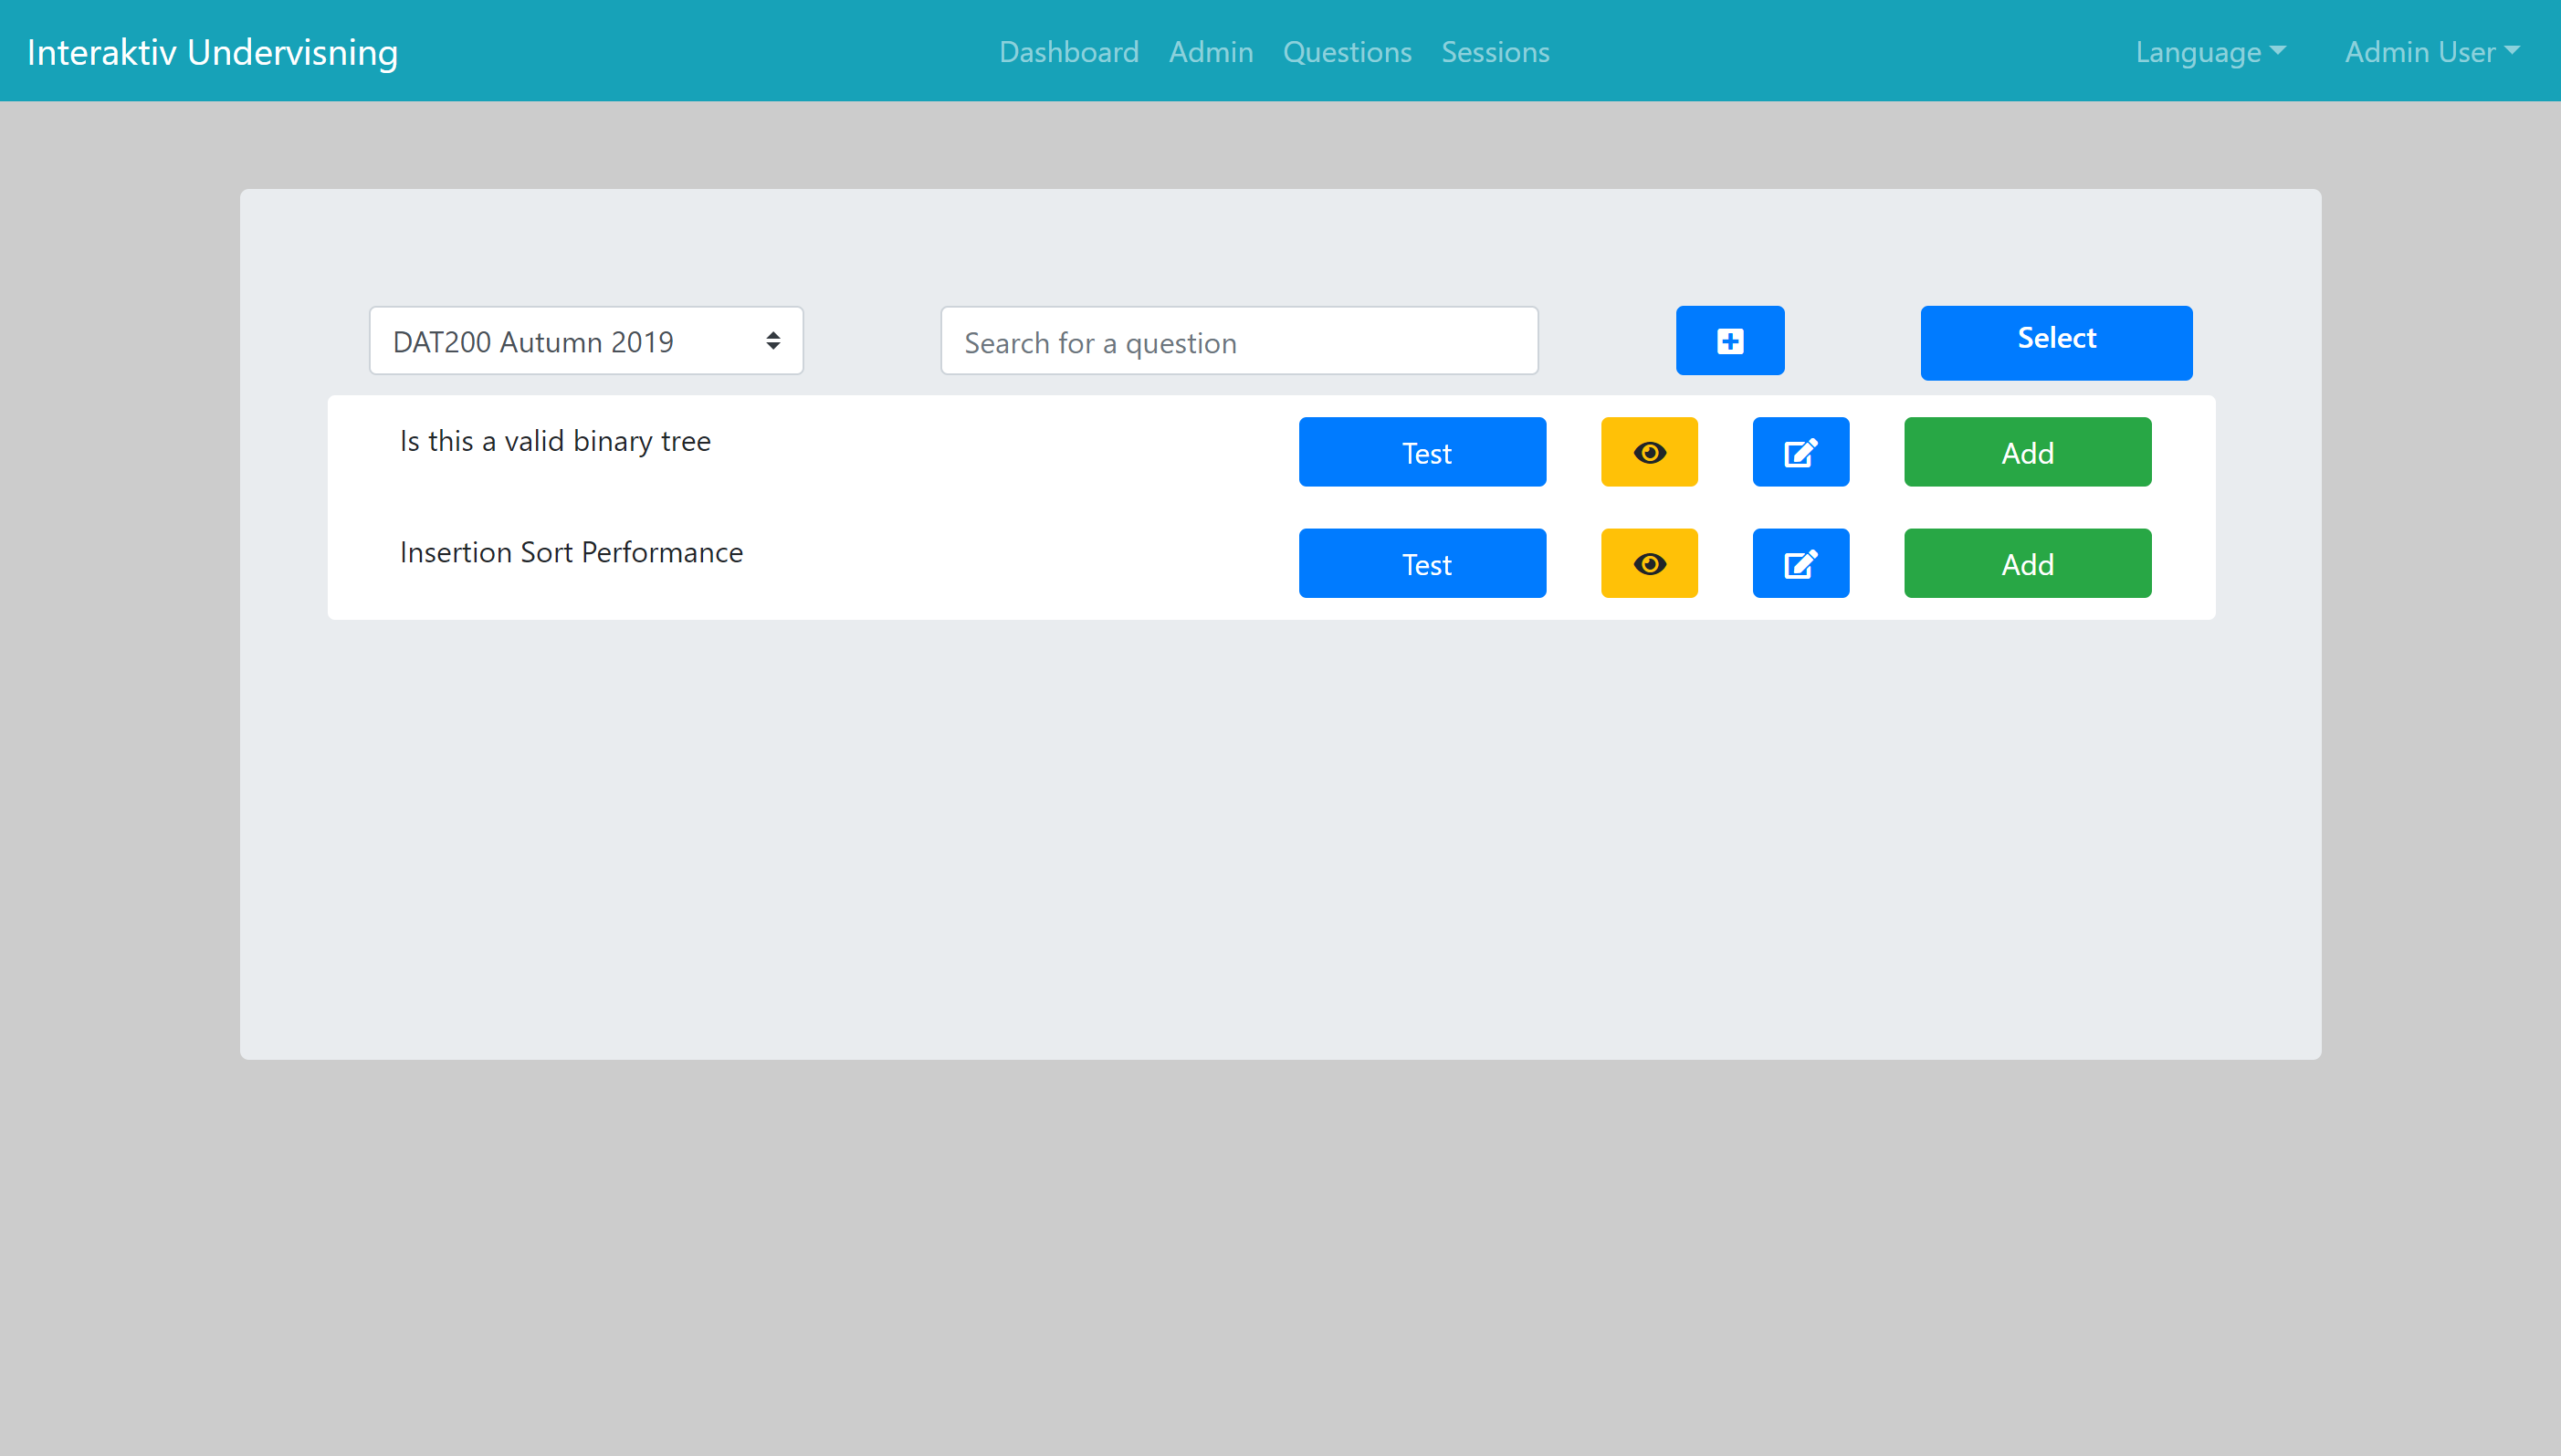
\includegraphics[width=0.80\linewidth]{/userManual/admin/QuestionDashboardWithQuestions}
    \caption{The figure displays an image of the Questions component.}
    \label{fig:questionVue}
\end{figure}
\noindent
Clicking the "+" button triggers the \code{showAddQuestionModal} method, allowing the EditQuestion component to be loaded in. This component contains a Bootstrap modal used for adding and editing question information. The main differences between the add and edit operations for the component are the following:
\begin{itemize}
\item[-] The edit functionality needs to load the question data from the database and fill in the forms with the correct information. 
\item[-] The request sent to the server contains the same question information, but the socket function that is triggered is different. The server functions are different primarily to distinguish between the insert and update SQL commands used on the database.
\end{itemize} 
The modal in EditQuestion is divided into three parts, namely Basic Information, Media and Solution type. The Basic Information part contains an input field for assigning the question title, a text area for giving a question description, a time input field and a time slider for assigning time. The fields use v-model to mount to the object \code{newQuestion}. A v-model is a two-way connection between a variable and a HTML element. The variable has to be a property on the \code{props} or the \code{data} object. This makes sure that if the variable value is changed either by functions or by user interaction, both will have access to the updated value.  The values assigned from the different form inputs are stored in the \code{data} property of the Vue context. The time slider and time input use different value formats, because of this, the time slider is linked with the \code{time} property. The time input uses a computed method (\code{timeInput}) to convert the \code{time} property to a text value. If the user changes the time input the computed method will convert it back to an integer value. This means that these elements always change their value depending on the other, resulting in them having the same value. If the time is set to “00:00”, then the question will not have a timer when used in a session. In the database, the value is stored as an integer, if the time value is 0, it is stored with a value of -1.
\\[11pt]
If the user uploads an image, the EditQuestion component the method \code{newFile} is triggered by an \code{onChange} event. The method validates the image because it is important to check that the file is an actual image file. If the validation passes, the image \code{File} object is converted into a buffer. This buffer, alongside the name, size and file type are pushed into a list as an object. When a question with an image is sent to the server, the image list is sent with the question information. On the server, it will first move the image buffer into a temporary list. Then the server creates file paths for each image and places them into the question object. After the question has been stored in the database, the image buffers are turned into image files and stored in the file system. Whenever a question is obtained from the database that has images, the server loads the images by using the file paths stored in the question object. When the image is going to be used on the client, a new buffer is created based on the image and stored in the question object. A question cannot have too many images assigned to it, as this would take up a lot of the needed data. The total amount of files attached to a question cannot exceed 1.5MB, and the user will get a warning once the amount exceeds 500KB. These checks will run in the validation once an image is added to the question. Images in a question are displayed as a preview with filename, file size, and a small image on the side.
\\[11pt]
Tables are added using 2-D lists where each element is a row. Each cell uses a HTML input field and has a v-model linking the value directly to the 2-D list. When displaying the 2-D list, each row and column is generated using a Vue feature called v-for. This feature allows HTML elements to be written once, and let a for loop generate the elements n times, based on the v-for input. The application also allows the addition of GraphDrawer drawings in an image format. When exporting a canvas element from the GraphDrawer as an image, a function \code{toDataURL} is called on the canvas element. The function returns a base64 data URL. Based on the information from this string an image object is created and added to the image list alongside images added by the user.
\\[11pt]
The solution type part focuses on determining the question type of the new question and for creating the question's solution. The type decides what format the question has for both the solution and for the client during a session. The solution to questions revolving data structures and algorithms is created on the server in the solution generator. The user only needs to give the necessary information for the question so that it is possible for the student to solve it, and for the server to be able to create the solution. There are two reasons for having the server handle the solution generation. The first reason is to keep it away from clients participating in a session. The second reason is that forcing the user to write the entire solution for every question would be rather tedious. Not to mention reducing the chances of having the solution being written incorrectly.
\begin{figure}[H]
	\centering
	\begin{subfigure}{0.45\linewidth}
        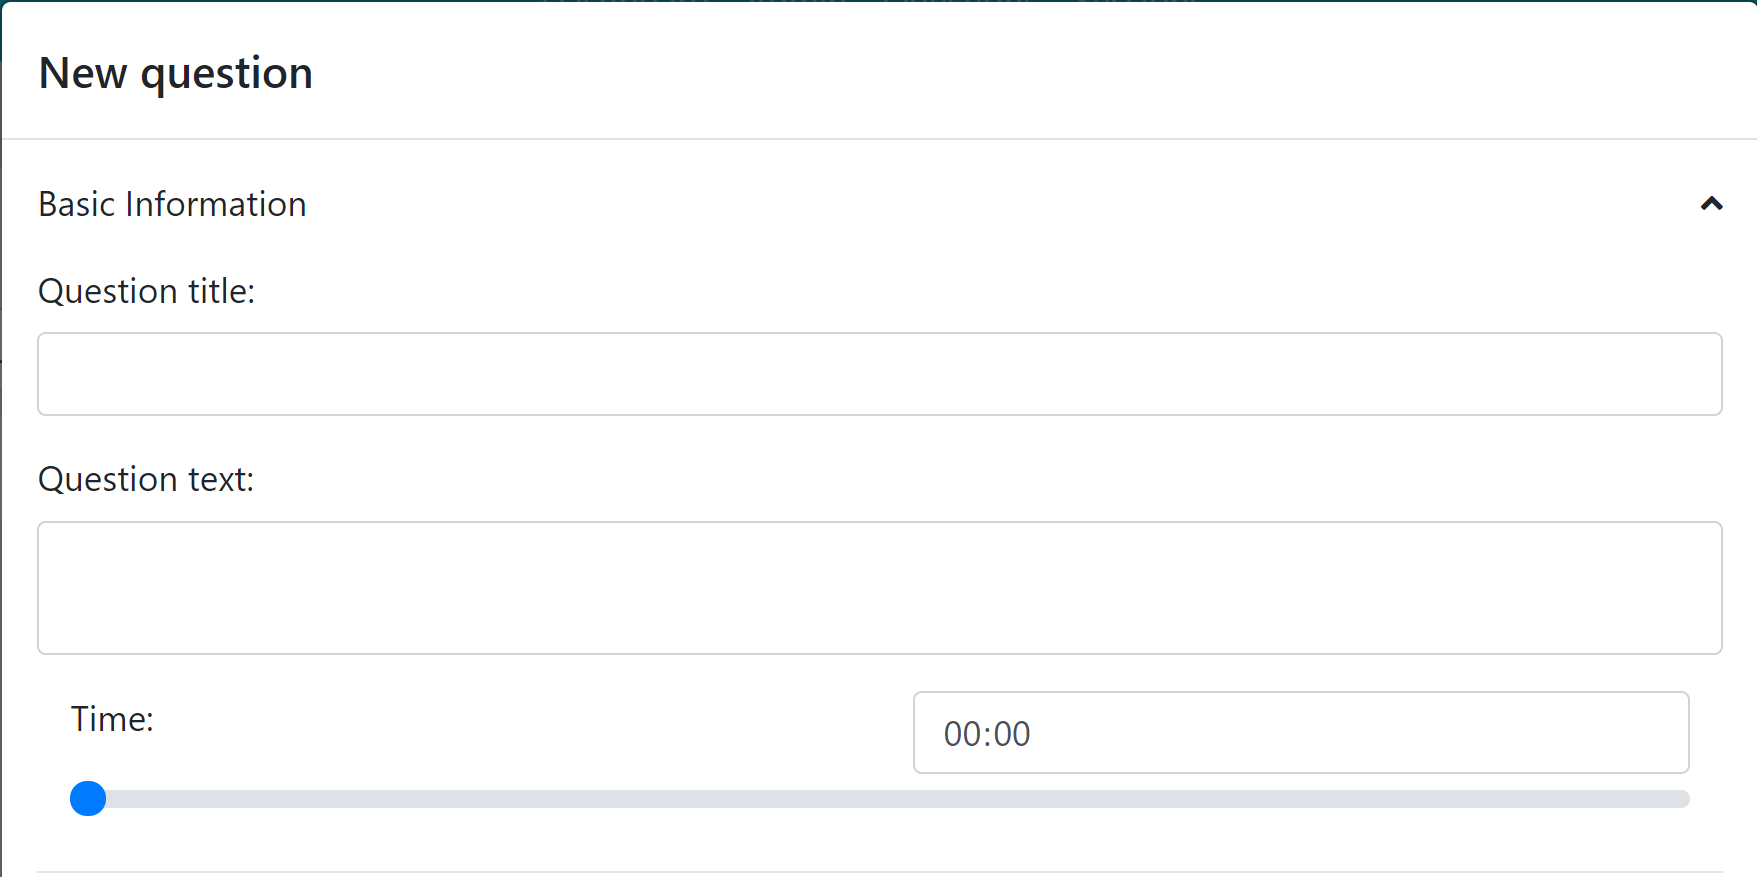
\includegraphics[width=\linewidth]{/userManual/admin/EditQuestionBasicInfo}
        \label{fig:editQuestionBasic}
	\end{subfigure}
	\hfill
	\begin{subfigure}{0.45\linewidth}
		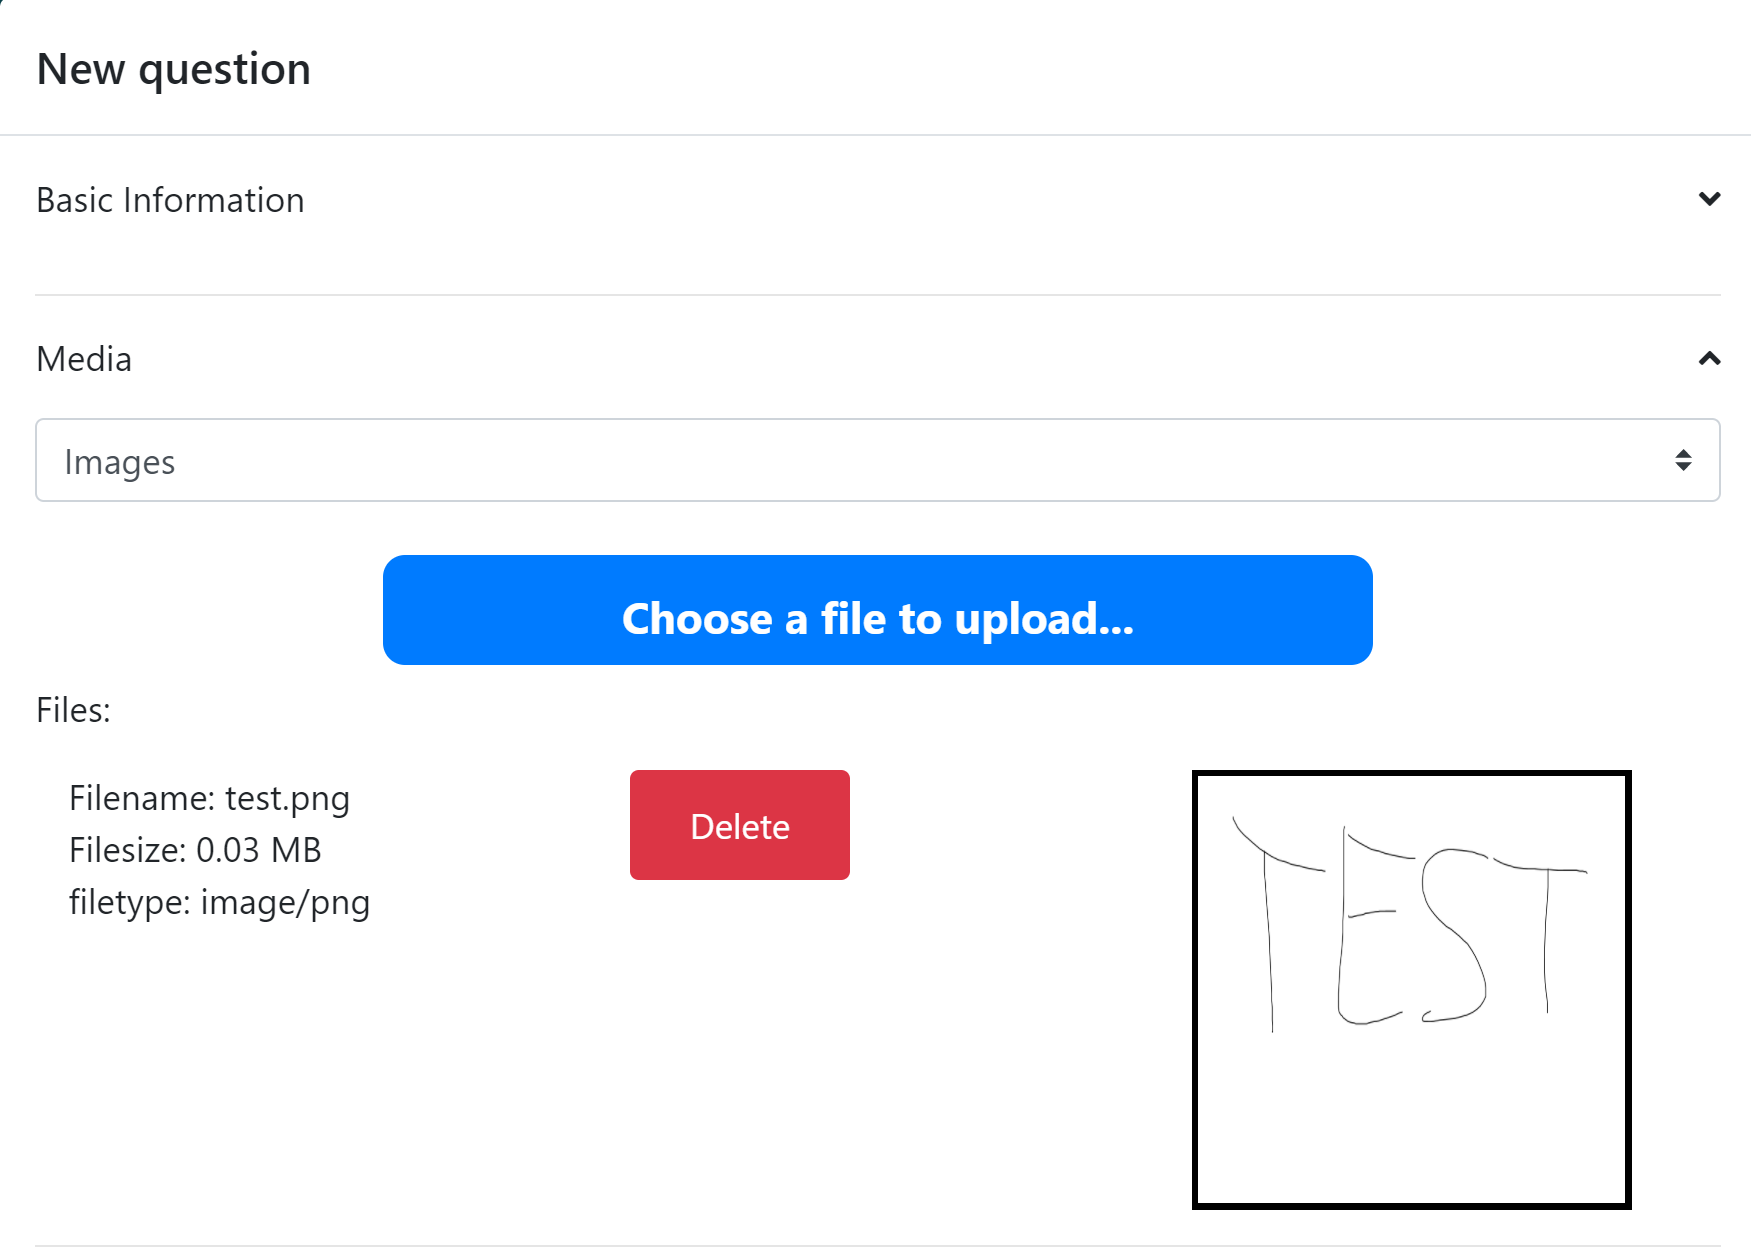
\includegraphics[width=\linewidth]{/userManual/admin/EditQuestionImageMediaPNG}	
		\label{fig:editQuestionMedia}
	\end{subfigure}
	\begin{subfigure}{0.45\linewidth}
		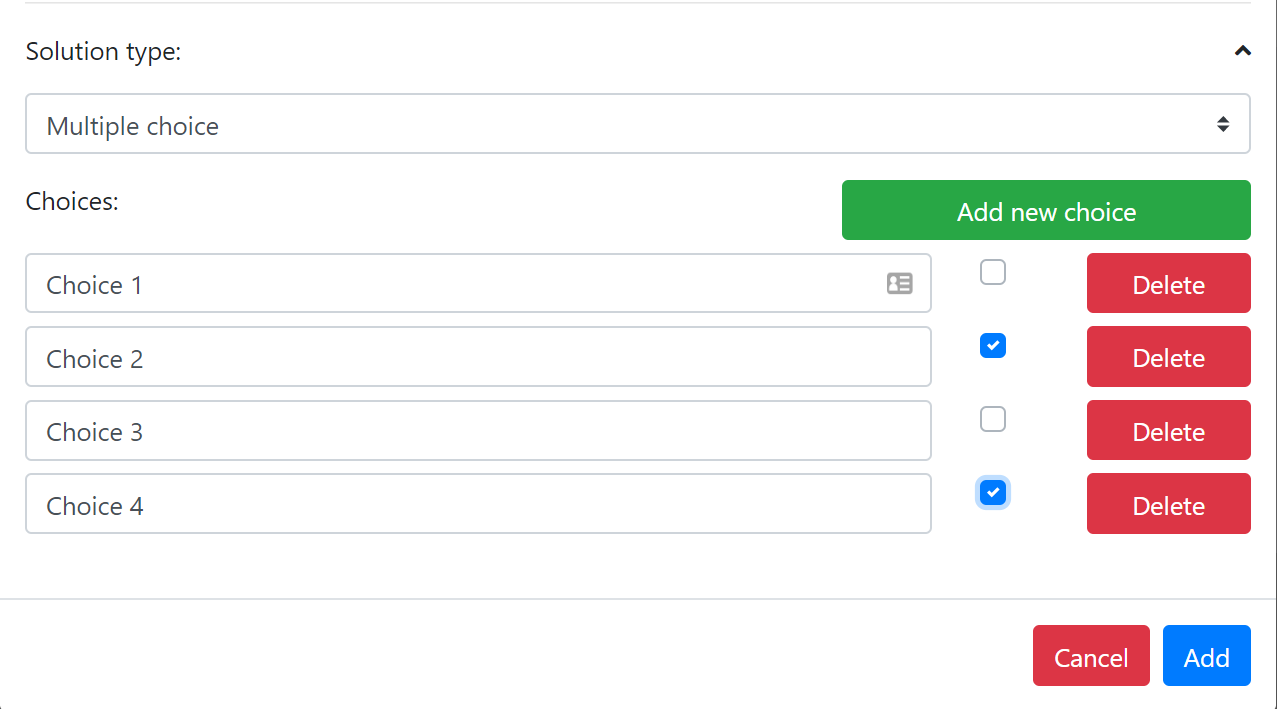
\includegraphics[width=\linewidth]{/userManual/admin/EditQuestionSolution}
		\label{fig:editQuestionSolution}
	\end{subfigure}
	\caption{These figures display sections of the EditQuestion component.}
	\label{fig:editQuestion}
\end{figure}
\noindent
When a user is finished creating a question, the question information is sent to the server through a socket request. The data sent to the server is the \code{newQuestion} object defined in the function \code{initializeState} in the component. Since all the properties in the \code{newQuestion} object are linked to the component, the server should have all the information it needs to generate the question solution. However, to avoid any problems regarding storing faulty questions on the server, the question information will first need to be validated by the server's validation checker. The user must at minimum fill in the information in a title, and the solution type with the solution properties for the wanted question to be valid. If the question information passes the validation checker, the question information and solution are inserted into the question table in the database. After the question is stored, socket messages are sent updating the question list on the client.
\\[11pt]
The question validation is divided into three script groups and linked together using a master script. The master script runs the validation for the first script group validating the basic information. The second script group runs the validation for any attached media. The third script group is the largest and runs validation on the solution. All script groups run even if the first group fails. If a group fails an error is pushed into a list containing all errors. After the master script is complete, the result is sent back to the client. If a check fails the error is displayed in a Bootstrap alert box informing the user what went wrong.
\\[11pt]
If the validation succeeds, then the information is sent to the solution generator that generates the appropriate solution in accordance with the question's type. The solution generator has a structure similar to that of the validation checker. Each solution generator has its own JavaScript file. The main "SolutionGenerator.js" file is used to link the question to its proper solution generator function. If the question requires the GraphDrawer tool to visualize its solution, then the solution object created from the generator is going to follow a certain format. The solution object here is an array that contains all the steps necessary to solve the exercise marked with a type property assigned with the action taken at the step. The last step is going to indicate either “finish” or “done” and is always going to be the last entry in the array. It is this object that is going to be used in the solution checker during an active session. The reason why this structure is used for solutions using the GraphDrawer, is because the GraphDrawer can show the entire process of solving the chosen exercise revolving an algorithm or a data structure.
\\[11pt]
If the user copies a question from one course to another course, all of the information is inserted to the database as a new question. This is done to prevent a change happening in one course affecting the question in the other course. A question cannot be deleted or edited after it has been used in a session. The reason for this is that the question information is still needed for Feide users to look at their previous participated sessions. If the question was to be removed after having been used in a session, then the student would not have access to the question information.
\\[11pt]
The question structure for this application was specifically chosen such that it would be easier for developers to implement and add new questions types. Excluding the work that is needed for writing the actual data structure or algorithm and its solution format, all that is required in order to add a new question type to a session is the following:
\begin{enumerate}
    \item Create a Vue component in both the questionResultScreenAnswer and questionResultScreenSolution directories. These are used for the DisplayQuestion component. The DisplayQuestion component is used for showing question results for each question.
    \item Add a b-form-group element to the EditQuestion component where only the necessary form items or Graphdrawer properties are set so that the user can create the new question type.
    \item If the question type requires certain unique information, then an extra property in the \code{newQuestion.objects} in the \code{initializeState} function should also be assigned and modeled appropriately to the HTML element in the form group.
    \item Add a JavaScript file in the validation checker for stopping illegal actions to the new type. 
    \item Implement the solution generator for the question type which is going to create the format for the solution object stored in the database.
    \item Add the new question type to question type array in the database.js file.
    \item Finally, implement a solution checker that is going to verify that the student answered the question correctly according to the solution object. 
    \item Add text to the locale files if the new question type requires them.
\end{enumerate}
